\chapter{Visualização e Análise de Dados}

\section{Visualização centralizada no Grafana}

A visualização dos dados de telemetria assume um papel crucial para a compreensão e monitorização eficaz de sistemas distribuídos. Embora as ferramentas Prometheus, Jaeger e Loki disponham de interfaces próprias para análise independente de métricas, \textit{traces} e \textit{logs}, a fragmentação das informações pode dificultar a correlação rápida entre estes dados. Por esse motivo, optou-se pelo Grafana como camada de visualização unificada, visando uma experiência integrada e eficiente. Entre as principais vantagens da utilização do Grafana destacam-se:

\begin{itemize}
\item A centralização das métricas, \textit{logs} e \textit{traces} num único painel interativo;
\item A capacidade avançada de correlação entre diferentes tipos de dados, facilitando a identificação de causas-raiz em anomalias;
\item A configuração unificada de alertas abrangendo todas as fontes de dados;
\item A interface intuitiva e personalizável, acessível a diferentes perfis técnicos;
\item Linguagens de consulta especializadas (\textit{PromQL}, \textit{LogQL}) diretamente integradas na ferramenta.
\end{itemize}

O Grafana habilita uma abordagem de ``\textit{single pane of glass}'', essencial para o acompanhamento consolidado do desempenho e da saúde do sistema. Além disso, permite seguir o percurso completo de uma requisição entre microsserviços e analisar a sua evolução temporal, proporcionando uma visão detalhada do comportamento distribuído da aplicação.



\break

\section{Organização dos Dashboards}

\subsection{Estrutura Lógica dos Dashboards}

Para garantir uma análise sistemática e eficiente dos dados recolhidos, a plataforma de visualização foi estruturada em diferentes painéis temáticos no Grafana. Esta organização permite um fluxo analítico claro, desde a observação de métricas de alto nível até à inspeção detalhada de eventos específicos, facilitando o diagnóstico rápido de anomalias e a compreensão do comportamento global do sistema.

De modo a assegurar uma exploração coerente e eficiente dos sinais de telemetria, os \textit{dashboards} foram agrupados em três categorias principais:

\begin{itemize}
    \item \textbf{Métricas da Aplicação.} Focadas no comportamento das APIs .NET, onde são monitorizados indicadores como o número de requisições HTTP por segundo, latência média e percentis (p95 e p99), taxas de erro (4xx e 5xx), bem como o consumo de CPU e memória por serviço. Estes painéis permitem identificar padrões de carga e avaliar a eficiência operacional dos microsserviços.
    
    \item \textbf{Infraestrutura Kubernetes.} Dedicados à monitorização dos recursos do cluster, através dos dados expostos pelo Node Exporter. Incluem métricas como utilização de CPU e memória por nó e por \textit{pod}, carga média do sistema (\textit{load average}), e capacidade e utilização de armazenamento. Estes dashboards fornecem uma visão sobre a saúde da infraestrutura e permitem antecipar situações de saturação ou falhas ao nível dos recursos físicos.
    
    \item \textbf{\textit{Logs} e \textit{Traces}.} Concebidos para análise detalhada de eventos e interações entre serviços. Nesta secção é possível filtrar \textit{logs} estruturados por nível de severidade, serviço ou mensagem, inspecionar \textit{spans} individuais e observar o encadeamento de operações entre microsserviços ao longo do tempo. Esta correlação entre \textit{ logs} e rastreamento distribuído suporta a identificação de pontos de falha, atrasos inesperados e comportamentos anómalos na comunicação entre componentes.
\end{itemize}

Esta estrutura modular facilita a navegação entre diferentes perspetivas operacionais e acelera o processo de diagnóstico e resolução de problemas. Para além disso, os dashboards incluem gráficos de séries temporais, indicadores numéricos e filtros dinâmicos, permitindo uma interpretação prática e contextual dos dados. Assim, a solução não apenas centraliza a telemetria, mas também proporciona aos engenheiros uma visão unificada e acionável sobre a saúde, desempenho e fiabilidade do sistema distribuído.

\subsection{Painéis de Dashboards e Metodologia de Análise}

A visualização de dados representa uma camada fundamental na estratégia de monitorização 
para sistemas distribuídos. Após a instrumentação e recolha dos sinais de telemetria, métricas, \textit{logs} e \textit{traces}, torna-se necessário disponibilizar uma interface 
capaz de sintetizar esta informação de forma clara, permitindo identificar rapidamente 
anomalias, diagnosticar problemas e interpretar o comportamento operacional das aplicações.

Nesta secção, apresentam-se os \textit{dashboards} desenvolvidos no Grafana para demonstrar a 
eficácia da solução proposta. O objetivo é ilustrar o percurso analítico completo, desde 
a deteção de um evento anómalo até à identificação da sua causa, evidenciando o valor 
prático da integração entre métricas, \textit{logs} e rastreamento distribuído.

Para efeitos de consistência e clareza, os exemplos apresentados focam-se exclusivamente no 
microsserviço \textit{TicketsManagement}.

Embora fosse possível incluir visualizações de outros serviços da arquitetura, tal abordagem tenderia a revelar informações redundantes, uma vez que os padrões e métricas observados seriam aplicáveis de forma semelhante. Assim, com esta escolha conseguimos proporcionar uma análise mais clara da \textit{pipeline} de monitorização em produção, evitando a dispersão do foco e privilegiando a profundidade sobre a generalidade.

\paragraph{1) Visão geral de \textit{logs} (ponto de partida).}

A Figura~\ref{fig:dash-1} apresenta uma visão agregada de \textit{logs} estruturados emitidos pelo 
serviço \textit{TicketsManagement}. Este painel permite observar o volume total de eventos, 
distribuição por severidade e principais \textit{endpoints} envolvidos. Este é o ponto de partida do processo analítico: permite perceber rapidamente se existem picos de erros, mensagens recorrentes ou padrões anómalos.

\begin{figure}[H]
    \centering
    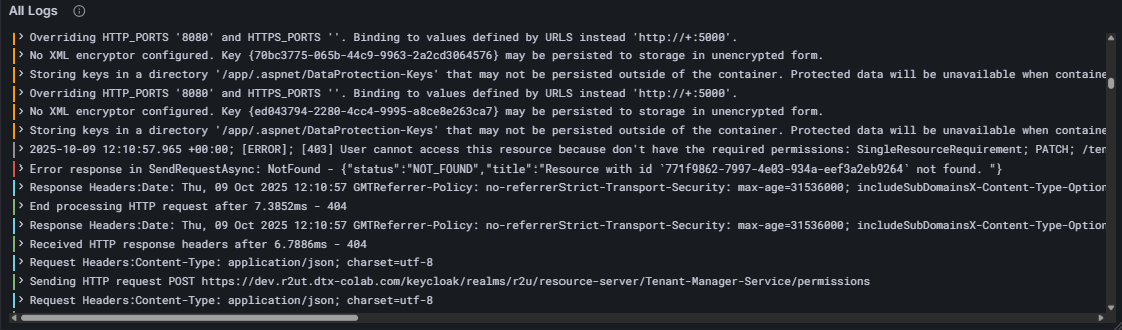
\includegraphics[width=\textwidth]{images/Grafana/all_logs_dashboard.png}
    \caption{Visão geral dos \textit{logs} estruturados do serviço \textit{TicketsManagement}.}
    \label{fig:dash-1}
\end{figure}

\textit{Transição:} Identifica-se um pico de erros ou eventos suspeitos e aplica-se filtragem 
por \texttt{service.name = TicketsManagement} e severidade (\texttt{ERROR}/\texttt{WARN}), avançando para o foco em erros.

\paragraph{2) Foco exclusivo nos erros.}

A Figura~\ref{fig:dash-2} mostra um painel dedicado exclusivamente a mensagens de erro, 
permitindo identificar \textit{endpoints} afetados, códigos HTTP e mensagens predominantes. 
Este painel acelera a identificação de falhas e reduz o \textit{MTTR} ao tornar evidentes os padrões de erro mais frequentes.

\begin{figure}[H]
    \centering
    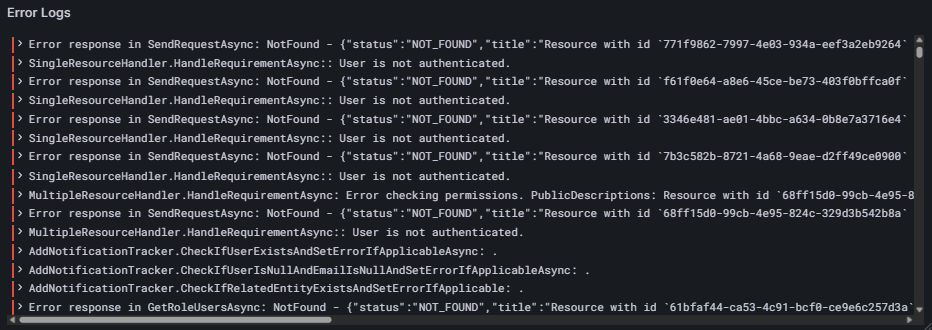
\includegraphics[width=\textwidth]{images/Grafana/error_logs_dashboard.png}
    \caption{Painel focado em \textit{logs} de erro do serviço.}
    \label{fig:dash-2}
\end{figure}

\textit{Transição:} Seleciona-se um evento concreto para análise detalhada do registo.

\paragraph{3) Expansão do registo e metadados.}

A Figura~\ref{fig:dash-3} apresenta o detalhe de um evento de \textit{log}, incluindo
\texttt{trace\_id}, \texttt{span\_id}, rota, código de estado e contexto adicional.

\begin{figure}[H]
    \centering
    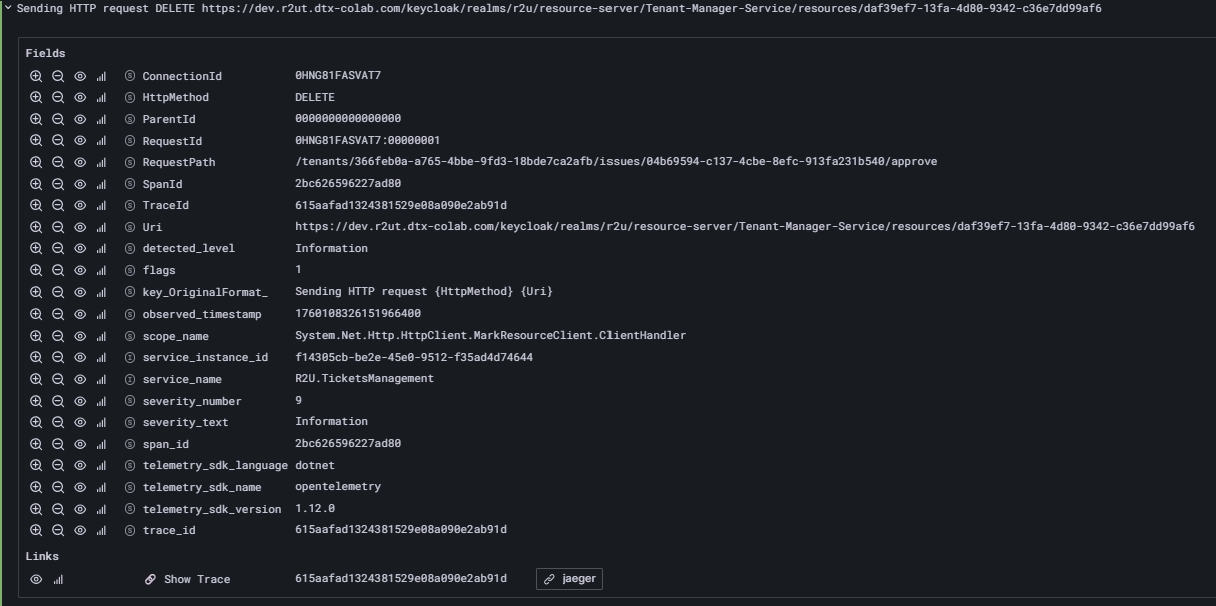
\includegraphics[width=0.9\textwidth]{images/Grafana/log_expanded.png}
    \caption{Detalhe de \textit{log} com metadados e referência direta ao \textit{trace}.}
    \label{fig:dash-3}
\end{figure}

\textit{Transição:} A partir do \texttt{trace\_id}, o analista segue para o rastreamento associado.

\paragraph{4) Métricas da aplicação.}

A Figura~\ref{fig:dash-4} apresenta indicadores operacionais da API: pedidos por segundo (RPS), distribuição por códigos HTTP, latência média e percentis (p95/p99). Este painel contextualiza o erro no panorama global do serviço: variações de latência ou picos de erros tendem a refletir-se aqui.

\begin{figure}[H]
    \centering
    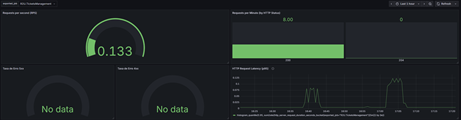
\includegraphics[width=\textwidth]{images/Grafana/metrics_dashboard.png}
    \caption{Métricas da aplicação: RPS, códigos HTTP, latência média e percentis.}
    \label{fig:dash-4}
\end{figure}

\textit{Transição.} Se houver degradação, o analista volta aos eventos e segue para o \textit{trace} para localizar gargalos. Em paralelo, valida se há limitação de recursos na infraestrutura.

\paragraph{5) Recursos da infraestrutura Kubernetes.}

A Figura~\ref{fig:dash-5} consolida métricas do cluster: utilização de CPU e memória por nó e por \textit{pod}, \textit{load average} e espaço de disco. Serve para confirmar ou excluir causas relacionadas com recursos (e.g., \textit{throttling}, saturação, \textit{out-of-memory}).

\begin{figure}[H]
    \centering
    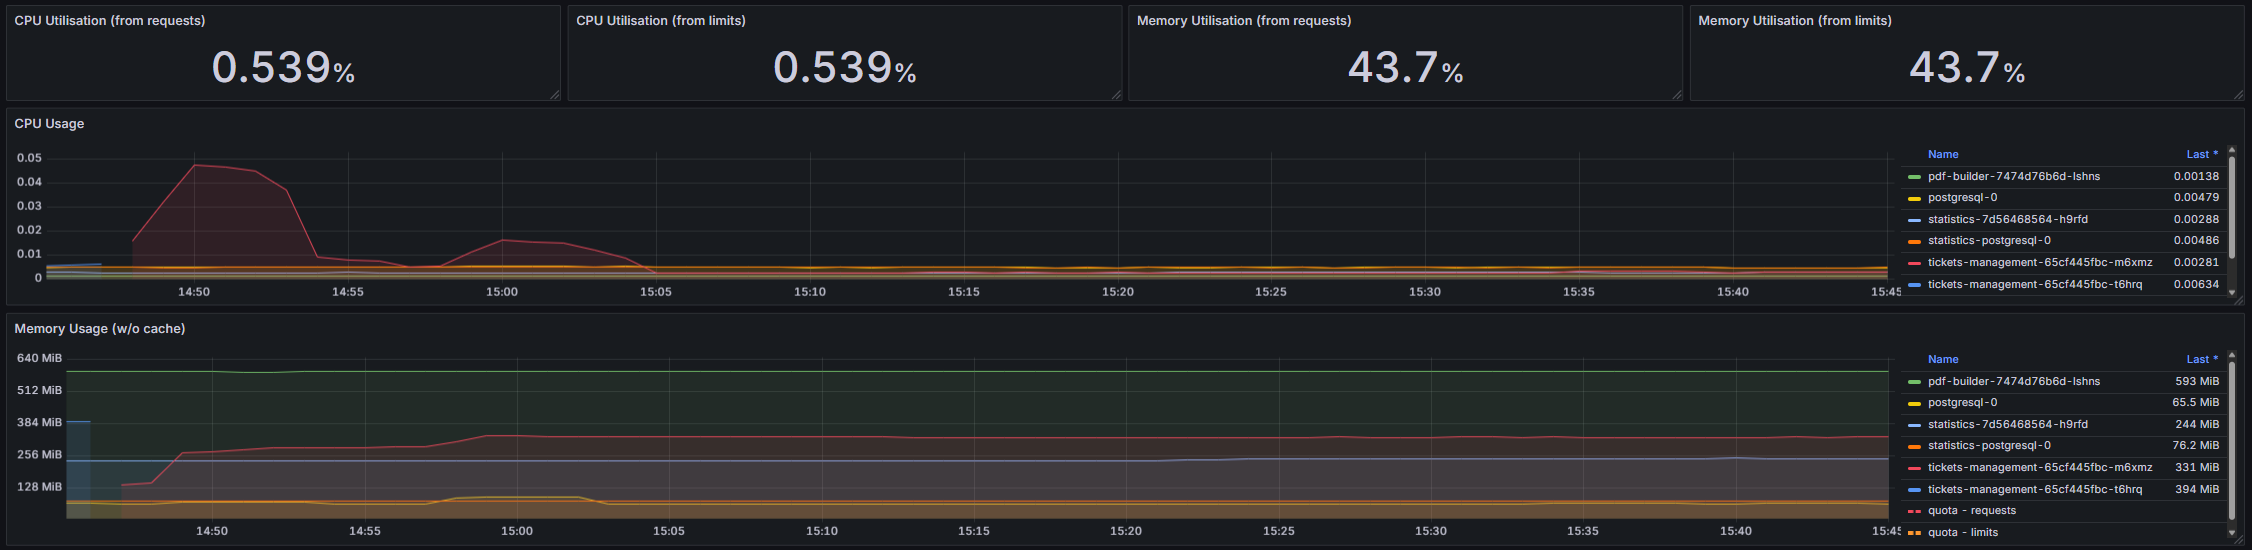
\includegraphics[width=\textwidth]{images/Grafana/cpu_memory_dashboard.png}
    \caption{Métricas de infraestrutura Kubernetes.}
    \label{fig:dash-5}
\end{figure}

 \textit{Transição.} Com os recursos estáveis, a investigação regressa ao encadeamento distribuído das chamadas para localizar a origem funcional do problema.

\paragraph{6) Rastreio distribuído.}

A Figura~\ref{fig:dash-6} ilustra um rastreamento completo associado ao incidente analisado. Observam-se as chamadas entre microsserviços, o tempo gasto em cada \textit{span} e a identificação de \textit{bottlenecks} (e.g., chamadas a \textit{databases} ou serviços externos).

\begin{figure}[H]
    \centering
    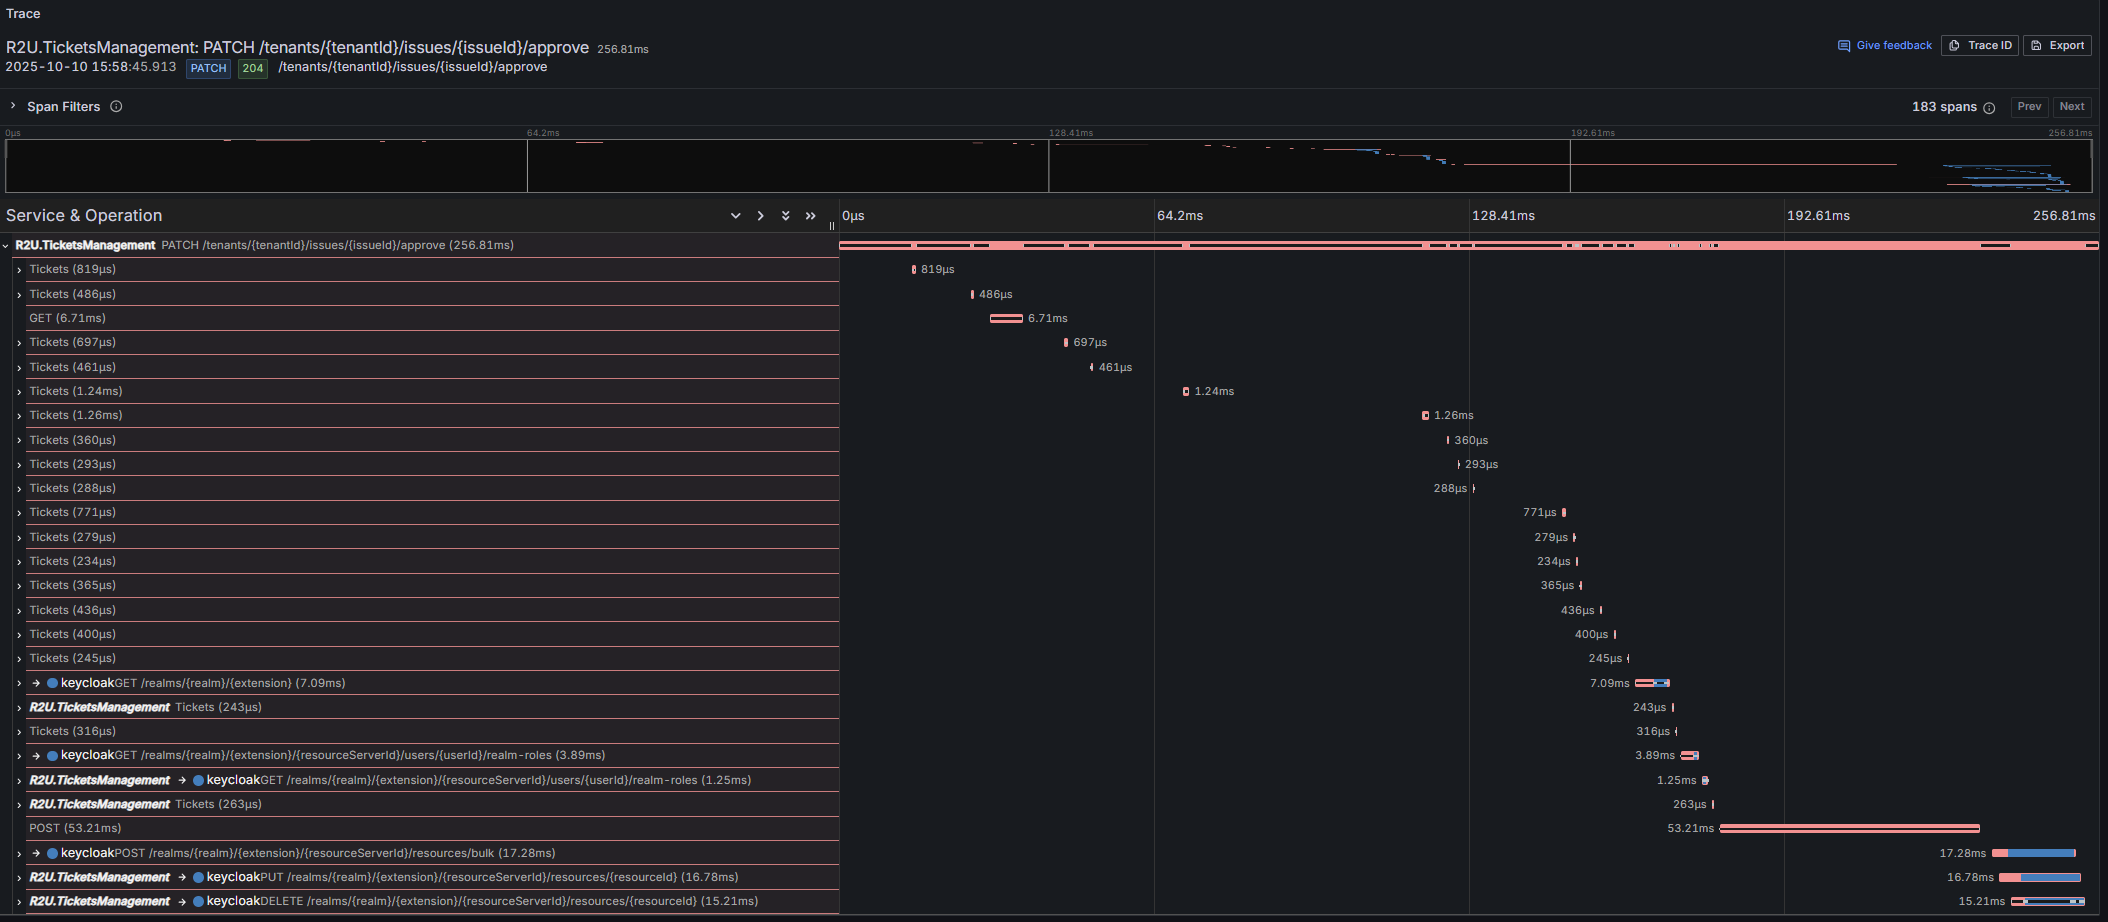
\includegraphics[width=\textwidth]{images/Grafana/trace_approve.png}
    \caption{Rastreamento distribuído associado ao evento analisado.}
    \label{fig:dash-6}
\end{figure}

\break

\subsection{Correlação entre \textit{Logs} e \textit{Traces}}

Um dos principais benefícios da solução implementada reside na correlação direta entre \textit{logs} 
e \textit{traces}. A Figura~\ref{fig:dash-7} apresenta um painel que liga cada registo de \textit{log} ao 
\textit{trace} correspondente, permitindo navegar rapidamente entre eventos e fluxos de execução.

\begin{figure}[H]
    \centering
    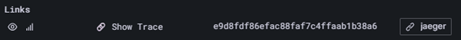
\includegraphics[width=0.8\textwidth]{images/Grafana/trace_link_por_log.png}
    \caption{Ligação direta do \textit{log} ao \textit{trace} correspondente.}
    \label{fig:dash-7}
\end{figure}

Esta funcionalidade acelera significativamente a deteção da causa raiz de incidentes, 
uma vez que permite cruzar mensagens de erro com a linha temporal e contexto completo 
da execução distribuída.

\paragraph{Nota sobre a migração da plataforma.}
Apesar da eficácia demonstrada, importa mencionar que a plataforma R2UT encontra-se ainda 
em fase de migração gradual para Kubernetes. Assim, apenas os serviços já migrados 
emitem telemetria compatível com o modelo adotado. À medida que a migração progride, a 
monitorização será estendida a toda a plataforma, permitindo rastreamento ponta-a-ponta.

\paragraph{Síntese do fluxo analítico.}
O processo recomendado segue a sequência:

\begin{enumerate}
\item Iniciar em \textit{logs} gerais (Figura~\ref{fig:dash-1}) e identificar picos;
\item Focar erros (Figura~\ref{fig:dash-2});
\item Expandir registo e seguir o \texttt{trace\_id} (Figura~\ref{fig:dash-3});
\item Validar métricas globais (Figura~\ref{fig:dash-4});
\item Confirmar estado da infraestrutura (Figura~\ref{fig:dash-5});
\item Inspecionar \textit{trace} completo (Figura~\ref{fig:dash-6});
\item Consolidar correlação (Figura~\ref{fig:dash-7}).
\end{enumerate}

Este método reduz o tempo de análise e materializa o Grafana enquanto \textit{single pane of glass} 
para operação e diagnóstico.


\section{Alertas e Notificações Operacionais}

A monitorização eficaz não se limita à visualização passiva de métricas, exige mecanismos de alerta que permitam atuação rápida perante degradações de desempenho, falhas de serviço ou comportamentos anómalos. Para esse fim, foi configurado o \textit{Prometheus AlertManager}, responsável por receber regras de alerta definidas no Prometheus e encaminhar notificações para canais operacionais pré-definidos.

Os alertas constituem um elemento crítico em ambientes \textit{cloud-native}, onde a natureza distribuída e dinâmica dos microsserviços pode levar a falhas rápidas e efeitos em cascata. Assim, foram definidas regras de monitorização orientadas a três objetivos principais: (i) assegurar disponibilidade, (ii) detetar degradação de desempenho e (iii) prevenir saturação de recursos.

A título ilustrativo, foram implementados alertas para as seguintes condições:
\begin{itemize}
    \item Taxa de erros HTTP 5xx superior a 5\% durante 5 minutos;
    \item Latência p95 das requisições superior a 1\,s;
    \item Utilização de CPU por \textit{pod} superior a 90\% durante período prolongado.
\end{itemize}

Embora o Grafana também suporte a configuração de alertas diretamente sobre \textit{dashboards}, a opção por utilizar o \textit{AlertManager} reflete as melhores práticas para ambientes de produção, privilegiando uma abordagem declarativa, versionável e escalável. As regras de alerta podem ser geridas em ficheiros YAML, permitindo a sua integração em pipelines CI/CD e garantindo consistência operacional.

No contexto prático deste trabalho, foi integrada uma notificação para o \textit{Slack}, garantindo que as equipas técnicas recebem alertas em tempo real num canal dedicado. Esta abordagem assegura visibilidade imediata sobre incidentes operacionais e permite resposta rápida, contribuindo para a redução do \textit{Mean Time to Detect} (MTTD) e do \textit{Mean Time to Recover} (MTTR).

A Figura~\ref{fig:slack-alerts} exemplifica dois alertas gerados pelo sistema: um associado a uma taxa de erros elevada e outro à utilização excessiva de CPU num \textit{pod} Kubernetes, ilustrando a capacidade do sistema em detetar e notificar eventos críticos.

\begin{figure}[H]
    \centering
    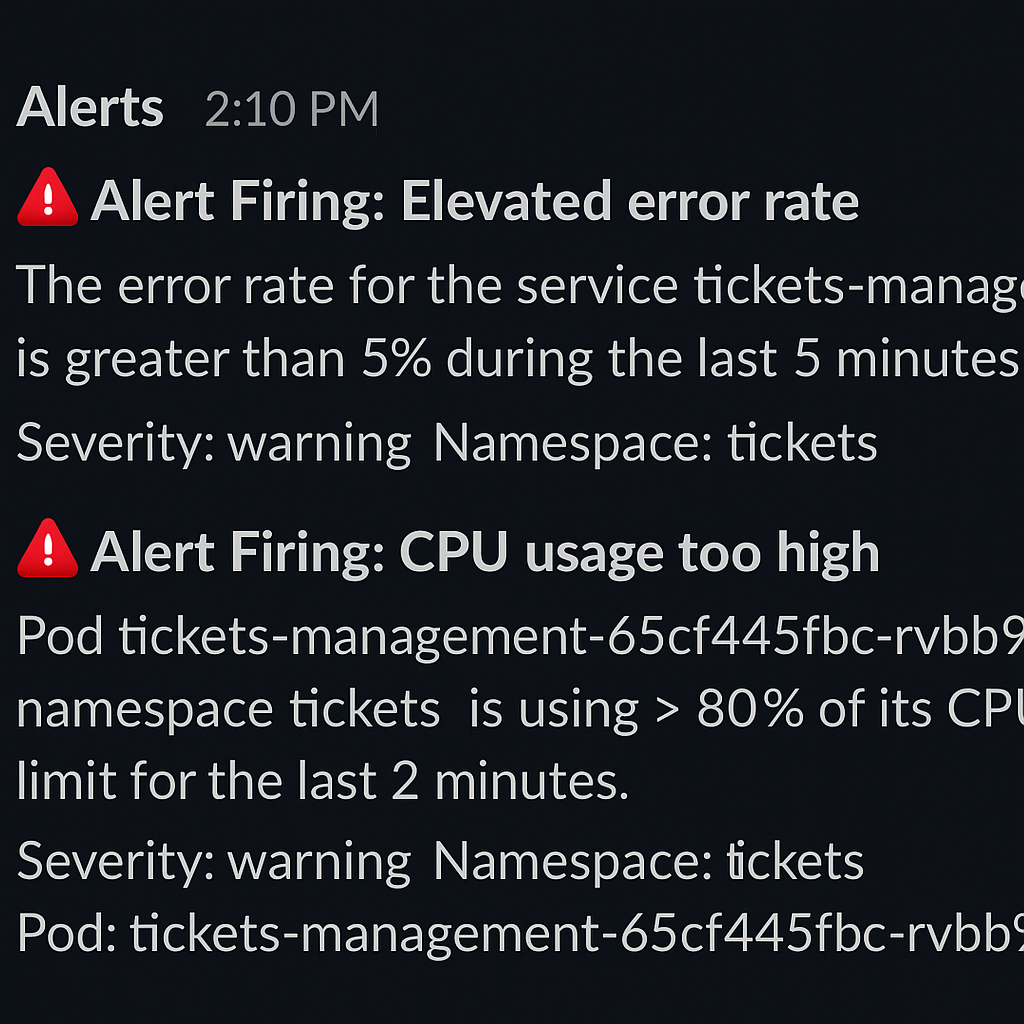
\includegraphics[width=0.5\textwidth]{images/Grafana/alertas.png}
    \caption{Notificações enviadas para o Slack contendo alertas gerados pelo \textit{AlertManager}, incluindo taxa de erros elevada e utilização excessiva de CPU.}
    \label{fig:slack-alerts}
\end{figure}


